
\chapter{BACKGROUND}
\label{chap:intro}
 
The presence of speech interference is a challenging issue for all automatic speech processing systems. 
As speech technology advances into our daily lives (in the form of text-to-speech recognition, speaker verification systems, etc.), the need to address multi-speaker interference increases. 
This increase is due to the number and amount of naturalistic human-to-human interactions captured for archiving, entertainment, social media, etc. 
In this study, multi-speaker interference is referred to as co-channel speech. 
Precisely, {\it co-channel speech} refers to single-channel audio data that contain more than one speaker. 
Channel, in our definition, is synonymous to {\it recording device}; hence single-channel implies access to only one recording. 
Unfortunately, due to the non-stationary nature of speech interference, co-channel speech is inherently a difficult type of signal for speech processing. 
The presence of multiple speakers in co-channel increases the complexity of problems that are already difficult to address in single speaker scenarios. 
However, advancements in single-speaker speech technology over the past two decades has allowed researchers to broaden their scope of interest. 
Today, automatic speech recognition (ASR) is enabled in most smart-phones. 
During the course of this study, both Microsoft Windows and Mac OS were released with built-in speech recognition capability and one comes with a voice-based user verification system. 
These signs reflect the reality that current speech technology is extending its reach into our daily activities. 
A significant portion of day-to-day speech data captured by devices is co-channel. 
This investigations is therefore partly due to the rise of a new age in speech technology where research is not limited to isolated single-speaker conditions. 

The focus of this study is to address various aspects of speaker recognition in co-channel speech data. 
This is accomplished by providing a clear definition of co-channel speech and its various forms. 
We will see that not only different solutions, but different approaches must be used to address each form of co-channel. 





A wide range of terms have been used to describe various aspects of co-channel speech, 
which will be clarified throughout this chapter. 
This study addresses both conversational speech and artificially mixed audio streams as co-channel. 
Although some studies propose multi-channel solutions to co-channel speech~\cite{panahi2009blind,xiao2011overlapped}, the focus here is solely on single-channel recordings (i.e., a single microphone). 
In co-channel data, a subset of instances may contain more than one ``active'' speaker at the same time, i.e. multi-speaker segments, 
which we label as ``overlapped speech''. 
Overlapped regions are segments of a co-channel signal where both speakers are simultaneously active. This categorization is summarized in Fig.~\ref{fig:cochannel_vs_overlap}.


\begin{figure}[h!]
	\centering
	\vspace{0mm}
	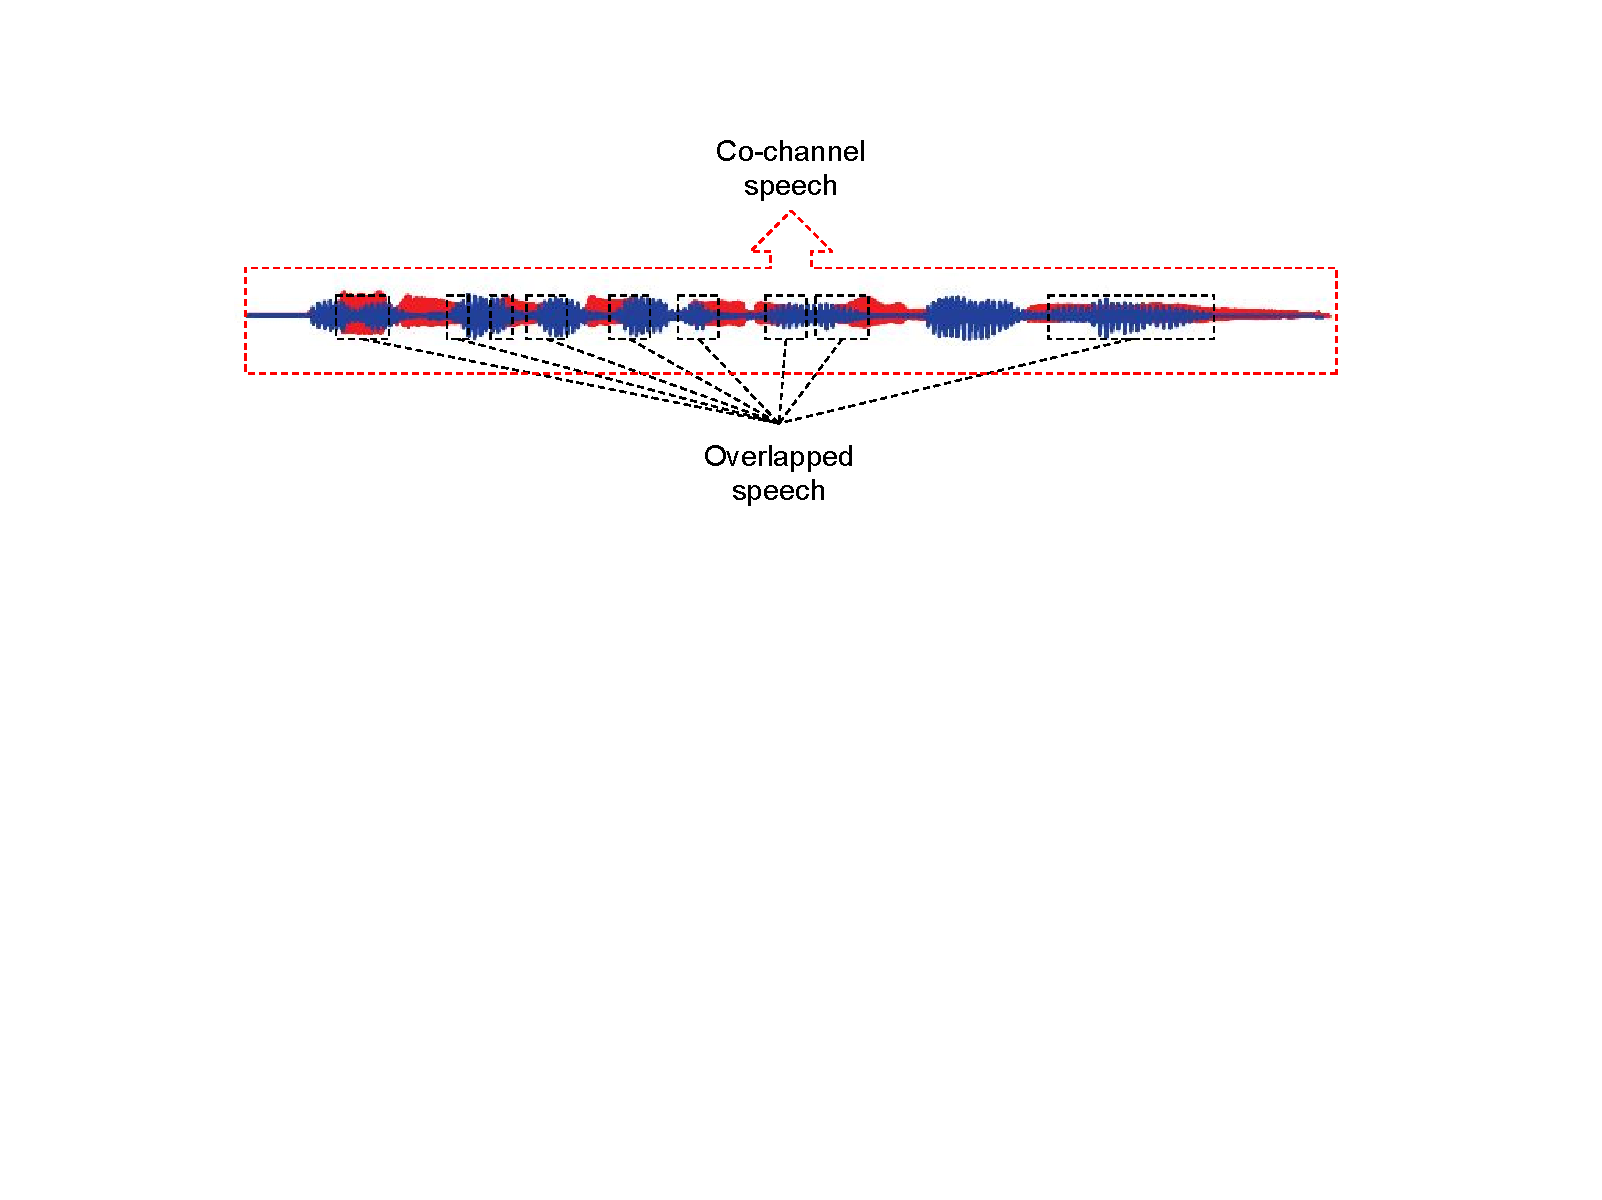
\includegraphics[height = 2in, width=0.9\textwidth]{figures/cochannel_vs_overlap-crop}
	\vspace{-3mm}
	\caption{\it \small Difference between co-channel and overlapped speech. Overlap refers to instances where more than one speaker is active. Co-channel is defined as an entire stream that contains multiple speakers. All co-channel files do not necessarily contain overlap. }
	\label{fig:cochannel_vs_overlap}
	\vspace{-3mm}
\end{figure}


%The specifics of recording conditions are overlooked in this study. 
%For example, information that relates to each speaker’s distance from the microphone and room acoustics. 
%This is intentional, since most of the difficulty in dealing with co-channel speech arises 
%from it being single-channel, which implies limited access to spatial 
%information as well as other sources of meta-data.

Aside from overlapped vs. non-overlapped speech, there are different ways of categorizing co-channel data in terms of how it is generated. 
Among such is a semantic classification that focuses on speakers' interactions with each other and divides co-channel data into two subgroups: 
\begin{itemize}
	\item conversational co-channel speech
	\item co-channel speech with independent parties (i.e., independent cross-talk)
\end{itemize} 

Conversational co-channel speech refers to recordings in which speakers acknowledge other parties in the recording and engage in dialog. 
Alterations of speech production are an important artifact of conversational co-channel speech, which are the result of conscious and unconscious reactions of the foreground speaker and interferer(s). 
Examples of such alterations are raised pitch and energy level ~\cite{Shriberg01observationson,schegloff2000overlapping}. 
Raised Pitch and volume are especially common at or around overlaps. 
Readers are probably familiar with political debates with heated arguments. 
Most debates are perfect instances of an exaggerated version of the above-mentioned changes in speech production. 
Schegloff argues that long and sustained overlaps are primarily a sign of argumentative speech~\cite{schegloff2000overlapping}. 
In such conversations, most speakers tend to alter their voice in order to control the floor. 
These changes are problematic in automatic speech applications and are considered a type of distortion. 
Treatments are directed towards applications that suffer the most from speech alterations, predominantly automatic transcription of speech, i.e., speech recognition. 
Aside from changes in speech production, the element of interference by competing speakers is also an important artifact observed during overlaps. 
Therefore, in conversational co-channel data, one has to consider both overlaps and speaker specific alterations as sources of distortion and mismatch. 

Co-channel data with independent parties, are examples of co-channel data where the speakers do not interact with each other. 
An example of this type is cross-talk between separate channels; imagine switching between radio stations on an analog AM radio. 
The main characteristic of such data is that speakers are not aware of each other and therefore do not pertain to normal conversational mannerisms. 
That includes following turn-taking rules, which in most cases limits overlapped speech. 
Artificially generated co-channel data (mixing independent channels) is another example of independent cross-talk. 
A considerable portion of this study will focus on this type of co-channel data to analyze performance of overlap detection and also speaker recognition. 
We rely on this type of data since it provides the flexibility of controlling the amount of overlapped speech. 
As we will show in the next chapter, conversational co-channel speech does not necessarily contain sufficient overlapped data for some of our experiments. 
Therefore, we allow ourselves to neglect some aspects of conversational co-channel speech for the benefit of more overlap. 
That is why we value ``co-channel data with independent parties'', despite some of its unrealistic characteristics compared to conversational speech. 

The treatment of different speech processing applications for co-channel speech will focus on one of the two categories described above. 
This study will focus on a number of speech applications including: 
\begin{itemize}
	\item Signal processing and audio classification: identifying and separating overlapped segments in co-channel files. 
	\item Speaker recognition/verification: The ability to automatically decide whether two or more speech samples belong to the same speaker. 
	\item Speaker diarization: Segmenting an audio stream by counting the number of speakers as well as determining who spoke when. 
\end{itemize}

A description of an outreach to signal processing in vehicles is also presented, where algorithms developed for co-channel speech analysis were used to improve driver safety. 

\section{Approach}

The goal of this thesis is to provide tangible solutions to problems caused by co-channel speech in automatic speaker recognition. 
We argue that part of these issues are caused by overlapped speech (direct speech interference), which plays a significant role in making co-channel speech a difficult problem. 
The presence of overlapped speech can be detrimental to speaker diarization and speech recognition systems. 
%There is no clear and unique way of labeling or transcribing overlapped segments. 
In speaker diarization, it becomes difficult to assess system performance at overlaps, due to the inherent ambiguity in labeling overlapped segments. 
The same goes for speech recognition where aside from determining which is the ``primary'' speaker, recognizing speech at overlaps is more difficult, due to interference coming from other speakers. 
For this and other reasons detailed in the next chapter, the first portion of this study is devoted to overlapped speech detection. 
Our approach to overlap detection will be to focus on developing signal processing techniques to detect and separate overlap from single-speaker speech. Figure~\ref{fig:overlap_applications} depicts some applications of overlap detection in speech technology. 

\begin{figure}[h!]
	\centering
	\vspace{0mm}
	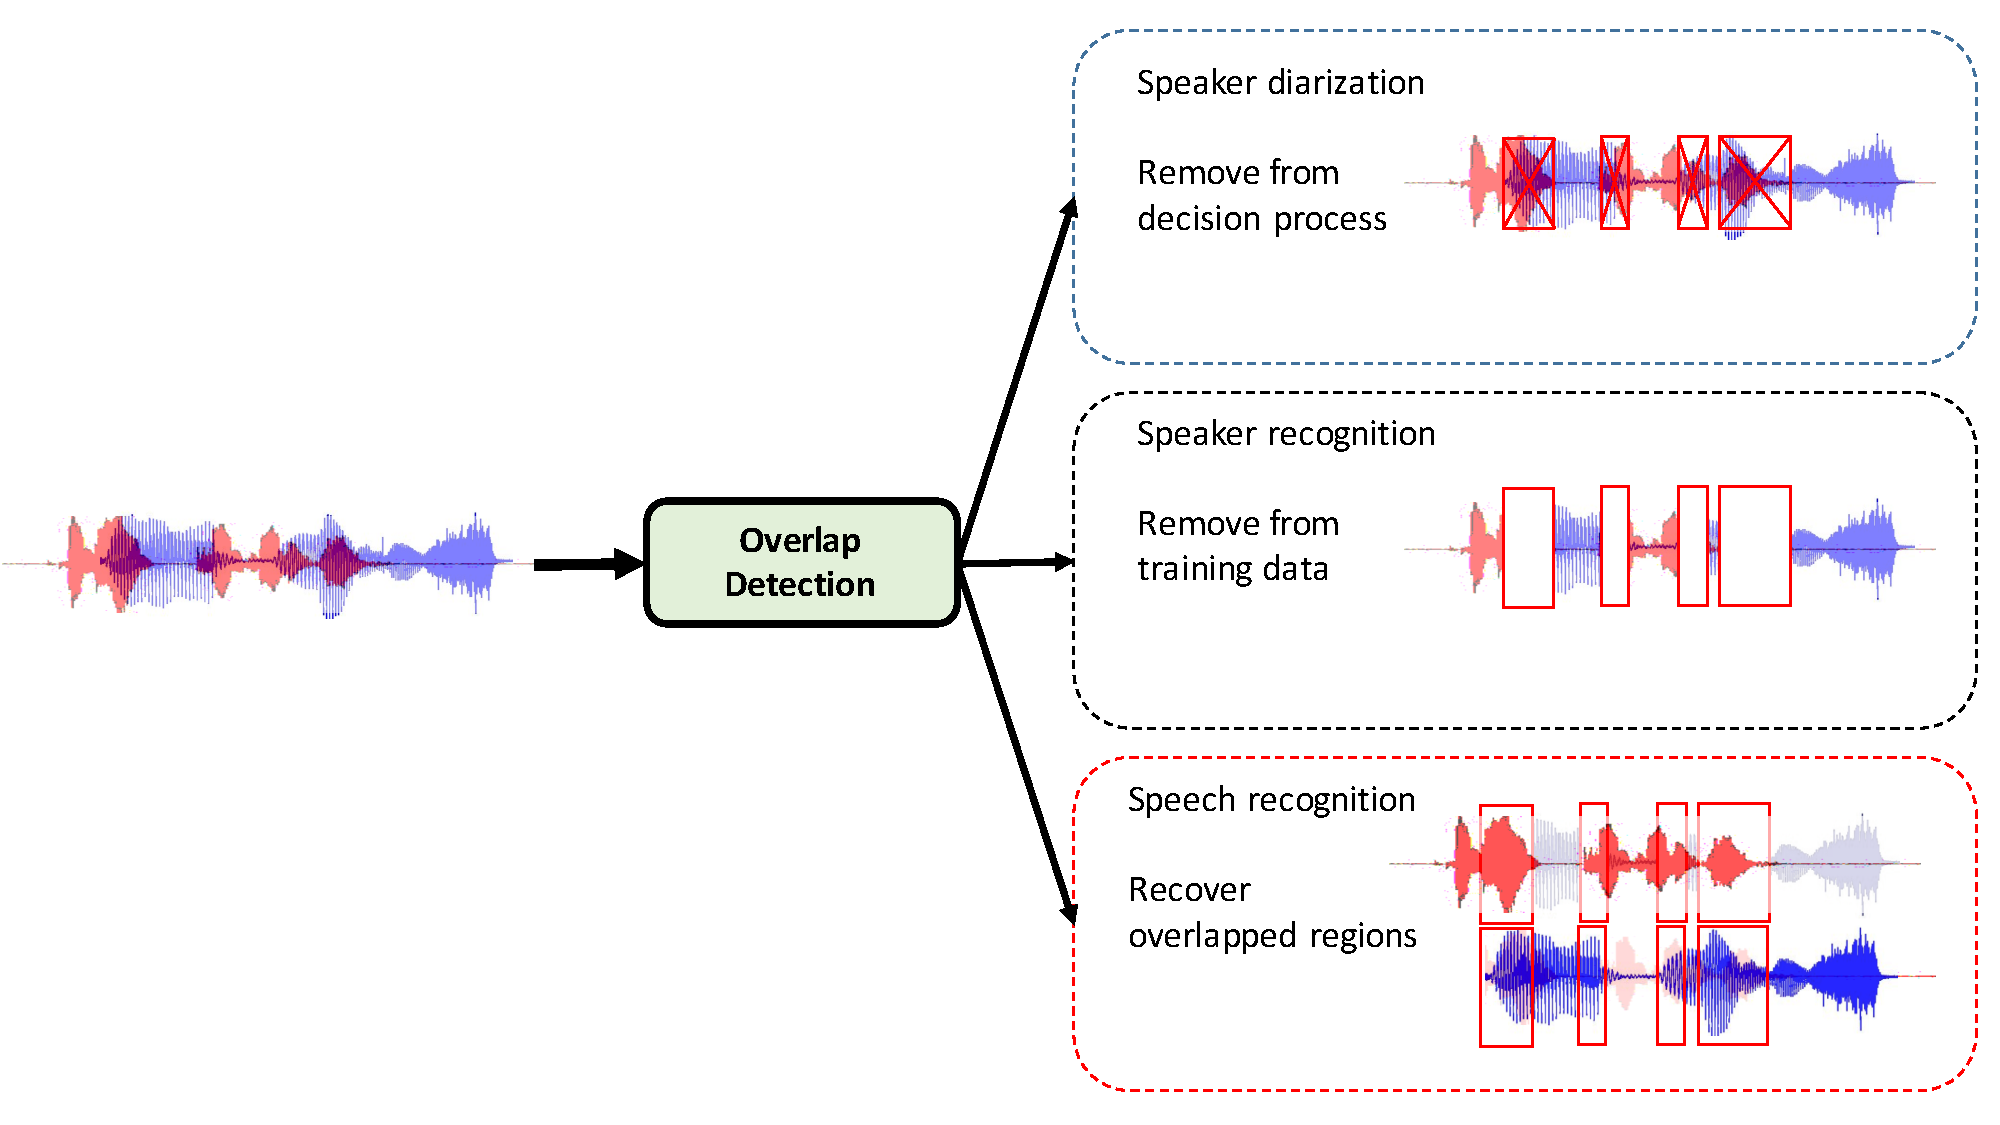
\includegraphics[height = 3in, width=\textwidth]{figures/overlap_detection_applications}
	\vspace{-3mm}
	\caption{\it \small Various applications of overlap detection. Top: In speaker diarization, ignoring overlapped regions provides a more fair assessment of diarization performance. Middle: Removing overlaps in speaker recognition increases the reliability of training data. Bottom: Overlap detection results can be used as an initial step to recover overlapped regions.}
	\label{fig:overlap_applications}
	\vspace{-3mm}
\end{figure}

Although overlap is considered an important aspect of co-channel speech, in many conversational speech data, the amount of overlap can be considered negligible, depending on the application. 
One such application is speaker recognition, which is also the main theme of this thesis. 
In text-independent speaker recognition, speech content (i.e., what is being said) is of less values compared to long-term speaker dependent characteristics (i.e., who is speaking). 
The standard approach in dealing with co-channel speech in such cases is speaker diarization. 
The role of diarization is to segment audio streams into shorter intervals each of which contains only one speaker. 
We consider speaker diarization a ``signal level'' approach. 
The term signal level is in respect to co-channel speech, since it is removed from the original signal prior to any other processing.
Alternately, a novel approach is presented in this study with the intention of bypassing the use of speaker diarization in the aforementioned scenario while preserving speaker recognition performance. 
This approach is to remove unwanted speaker-dependent information from latent variable subspaces generated from audio files~\cite{dehak2011front,kenny2010bayesian}. 
We refer to such solutions as ``subspace level''. 
Therefore, Chapters~\ref{chapter:backend}~and~\ref{chap:spkr_diar} each propose a different approach to remove interfering speakers from co-channel data. 
\begin{enumerate}
\item Remove interfering speakers in the feature subspace level: i-vector subspace factorization.
\item Remove interfering speakers in the signal level: speaker diarization.
\end{enumerate}

Speaker diarization, will attempt to recognize and group speech that belongs to the same speaker in a co-channel audio stream. 
While subspace factorization maps speaker-dependent models to a subspace that will only contain parameters identifying the speaker of interest (aka primary speaker). 
Once again it should be pointed out that the main theme of this study is to address speaker recognition and identification in co-channel speech. 
Which makes speaker diarization an inseparable part of our approach. 


\section{Outline}
\label{sec:intro_outline}
This dissertation is organized in the following manner. 
Thesis contributions are split into two main categories: 1) signal processing approaches, 2) probabilistic modeling. 
Chapter~\ref{chapter:front-end}, overlap detection methods, presents signal processing techniques used for overlap detection. 
Chapter~\ref{chapter:ovl_in_sid}, speaker recognition in overlapped speech, highlights the importance of addressing overlapped speech in speaker recognition problems. 
In addition, techniques proposed Chapter~\ref{chapter:front-end} are used in Chapter~\ref{chapter:ovl_in_sid} to improve recognition performance. 
Chapter~\ref{chapter:backend}, speaker recognition in co-channel speech, focuses on probabilistic modeling techniques to improve speaker recognition in co-channel. 

In addition to the two primary contributions, this thesis also covers practical aspects of co-channel speech processing. 
These aspects are covered in two frameworks. 
The first is the description of CRSS-SpkrDiar (Chapter~\ref{chap:spkr_diar}), which is an end-to-end speaker diarization system. 
The second aspect is an exhibition of interdisciplinary applications of co-channel speech  in other signal processing applications (Chapter~\ref{chap:applications}). 

Finally, a summary of conclusions and references to future studies are presented in Chapter~\ref{chapter:conclusions}. 

\section{Thesis Contributions}
\label{sec:contributions}
This dissertation investigates various aspects of co-channel speech and is novel in a number of ways. 
The most important contribution is to:
\begin{itemize}
	\item separate overlapped speech from co-channel.
\end{itemize}
The significance of this contribution is in its different perspective compared to existing studies. 
Solely focusing on overlap instead of co-channel (or vise versa) limits the applicability of methods and makes it difficult to compare studies, since different studies refer to different phenomena as co-channel. 

The second contribution is in the signal processing perspective, which is to
\begin{itemize}
	\item propose features to detect overlapped speech from single-speaker speech (overlapped speech detection).
\end{itemize}
This is important, since overlap detection constitutes a significant portion of co-channel research. 
Being able to detect overlapped segments is also useful in other problems related to co-channel analysis. 
One of the applications of overlap detection in co-channel speech is used in speaker diarization systems. 
The contribution in regards to speaker diarization is to:
\begin{itemize}
	\item provide a detailed description of CRSS-SpkrDiar, a speaker diarization tool-kit. 
\end{itemize}
The last contribution of this study focuses on latent space analysis, which is to:
\begin{itemize}
	\item develop and analyze modified probabilistic linear discriminant analysis to suppress interfering speech to improve speaker recognition performance. 
\end{itemize}
The theme in all of the aforementioned contributions is speaker recognition. 
Therefore, all of the techniques and analyses provided in the next chapters are in accordance with speaker recognition frameworks and are intended to improve speaker recognition performance. 